\appendix

\section{Appendiks - V-modellen}\label{app:vmodell}

V-modellen er illustrert i figur~\ref{fig:V-Modellen} Det kan være fristende å hoppe direkte inn i implementasjonsfasen, men dere bør ikke ta for lett på hverken analyse og design, eller testing. Det er mye bedre med noen få linjer gjennomtenkt og veltestet kode, enn mange linjer med \textit{spaghetti-kode}.

\begin{figure}[ht]
    \centering


\resizebox{1\textwidth}{!}{

\tikzset{every picture/.style={line width=0.75pt}} %set default line width to 0.75pt        

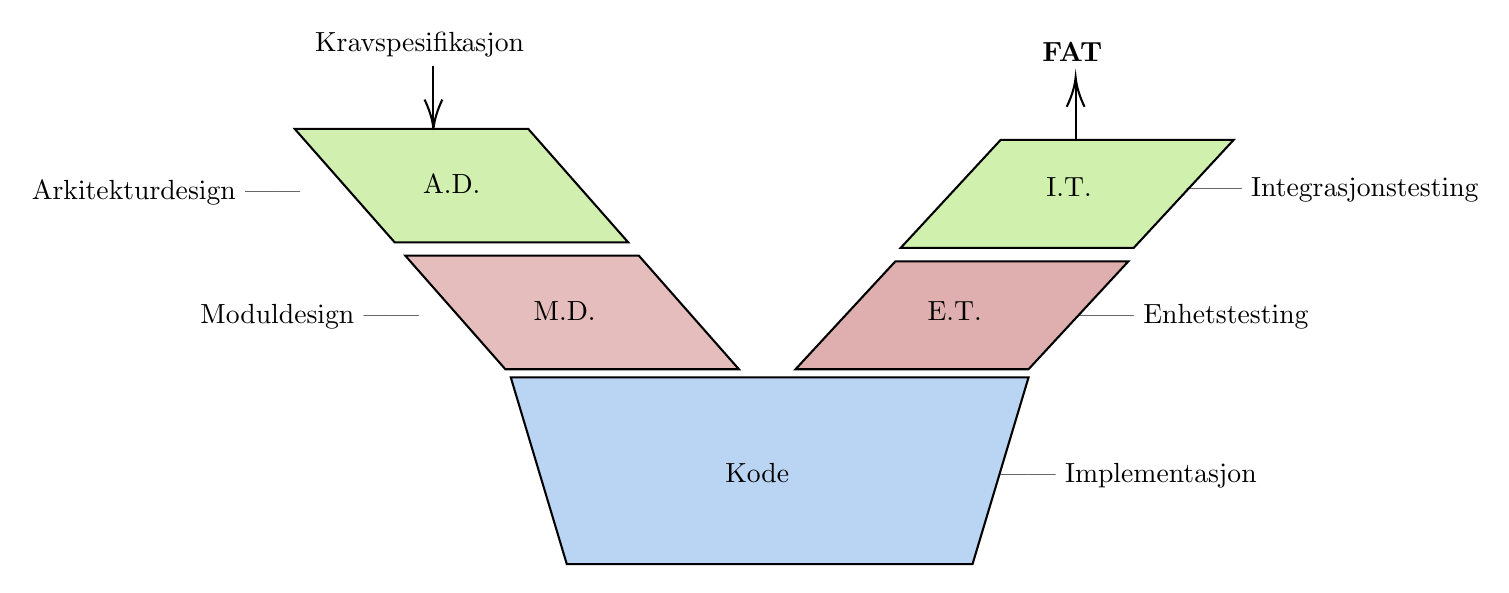
\begin{tikzpicture}[x=0.75pt,y=0.75pt,yscale=-1.3,xscale=1.3]
%uncomment if require: \path (0,300); %set diagram left start at 0, and has height of 300

%Shape: Trapezoid [id:dp9397778815056024] 
\draw  [fill={rgb, 255:red, 186; green, 212; blue, 243 }  ,fill opacity=1 ] (402.56,179.2) -- (381.8,248.4) -- (231.41,248.4) -- (210.65,179.2) -- cycle ;
%Straight Lines [id:da45606788276056864] 
\draw    (182,64) -- (182,85.2) ;
\draw [shift={(182,87.2)}, rotate = 270] [color={rgb, 255:red, 0; green, 0; blue, 0 }  ][line width=0.75]    (10.93,-3.29) .. controls (6.95,-1.4) and (3.31,-0.3) .. (0,0) .. controls (3.31,0.3) and (6.95,1.4) .. (10.93,3.29)   ;
%Straight Lines [id:da6815083924467882] 
\draw    (420,70) -- (420,91.2) ;
\draw [shift={(420,68)}, rotate = 90] [color={rgb, 255:red, 0; green, 0; blue, 0 }  ][line width=0.75]    (10.93,-3.29) .. controls (6.95,-1.4) and (3.31,-0.3) .. (0,0) .. controls (3.31,0.3) and (6.95,1.4) .. (10.93,3.29)   ;
%Shape: Parallelogram [id:dp15304372294969504] 
\draw  [fill={rgb, 255:red, 223; green, 175; blue, 175 }  ,fill opacity=1 ] (353.21,136.2) -- (439.56,136.2) -- (402.55,176.2) -- (316.2,176.2) -- cycle ;
%Shape: Parallelogram [id:dp7976543176271034] 
\draw  [fill={rgb, 255:red, 208; green, 240; blue, 173 }  ,fill opacity=0.98 ] (130.56,87.1) -- (217.11,87.1) -- (254.2,129.2) -- (167.65,129.2) -- cycle ;
%Shape: Parallelogram [id:dp7576209688334508] 
\draw  [fill={rgb, 255:red, 229; green, 189; blue, 189 }  ,fill opacity=1 ] (171.56,134.1) -- (258.11,134.1) -- (295.2,176.2) -- (208.65,176.2) -- cycle ;
%Shape: Parallelogram [id:dp6876146189594805] 
\draw  [fill={rgb, 255:red, 208; green, 240; blue, 173 }  ,fill opacity=1 ] (392.21,91.2) -- (478.56,91.2) -- (441.55,131.2) -- (355.2,131.2) -- cycle ;

% Text Node
\draw (289,210) node [anchor=north west][inner sep=0.75pt]   [align=left] {Kode};
% Text Node
\draw (364,150) node [anchor=north west][inner sep=0.75pt]   [align=left] {E.T.};
% Text Node
\draw (177,103) node [anchor=north west][inner sep=0.75pt]   [align=left] {A.D.};
% Text Node
\draw (391,210) node [anchor=north west][inner sep=0.75pt]   [align=left] {------ Implementasjon};
% Text Node
\draw (420,151) node [anchor=north west][inner sep=0.75pt]   [align=left] {------ Enhetstesting};
% Text Node
\draw (460,104) node [anchor=north west][inner sep=0.75pt]   [align=left] {------ Integrasjonstesting};
% Text Node
\draw (94.5,151) node [anchor=north west][inner sep=0.75pt]   [align=left] {Moduldesign ------};
% Text Node
\draw (32,105) node [anchor=north west][inner sep=0.75pt]   [align=left] {Arkitekturdesign ------};
% Text Node
\draw (137,50) node [anchor=north west][inner sep=0.75pt]   [align=left] {Kravspesifikasjon};
% Text Node
\draw (406.5,54) node [anchor=north west][inner sep=0.75pt]   [align=left] {\textbf{FAT}};
% Text Node
\draw (218,150) node [anchor=north west][inner sep=0.75pt]   [align=left] {M.D.};
% Text Node
\draw (408,104) node [anchor=north west][inner sep=0.75pt]   [align=left] {I.T.};


\end{tikzpicture}}
    \caption{Illustrasjon av V-modellen.}
    \label{fig:V-Modellen}
\end{figure}


\subsection{Arkitekturdesign}

Det aller viktigste er at man faktisk forstår kravene i spesifikasjonen. Når man først er sikre på hva som kreves av slutt-systemet, burde man tenke gjennom hvilke implikasjoner dette har for koden som skal skrives senere.

På dette stadiet ønsker vi å bestemme en \textit{arkitektur} som vil oppfylle kravene fra spesifikasjonen. Dette innebærer å legge abstraksjonsnivået forholdsvis høyt, og ignorere implementasjonsdetaljer enn så lenge.

\textbf{Eksempel}: Heisen skal kunne huske ordre helt til de blir ekspedert. Ikke tenk: \textit{Dette skal jeg implementere som en lenket liste}, men heller: \textit{På arkitekturnivå trenger vi et køsystem}. Detaljer om hvordan et eventuelt køsystem er implementerert kommer ikke inn i bildet på dette stadiet.

Resultatet av dette stadiet bør være ett eller flere klasse-diagrammer som illustrerer hvilke moduler styringssystemet skal bestå av. For å få en ide om hvilken funksjonalitet hver modul må tilby, kan det også være lurt å sette opp et par sekvensdiagrammer som illustrerer hvordan forskjellige moduler samarbeider. i tillegg, kan man også benytte kommunikasjons-diagrammer for å gi en bedre oversikt over grensesnittet mellom hver modul.

\subsection{Moduldesign}
Når man har en overordnet tanke over hvilke moduler som kreves for å oppfylle kravspesifikasjonen, er det på tide å skissere hvordan hver modul skal se ut. Et spørsmål som er lurt å ta stilling til her er om hver modul trenger å lagre tilstander eller ikke.

\textbf{Eksempel}: Et kø-system trenger åpenbart å lagre tilstand, mens en modul som utelukkende setter pådrag til motor-styringsboksen kanskje kan skrives uten å ha hukommelse.

En modul som ikke trenger å lagre tilstander vil alltid ha færre måter den kan feile på enn en tilsvarende modul som lagrer tilstand. Det kan derfor være lurt å skille ut delene av systemet som har denne funksjonaliteten i en dedikert tilstandsmaskin, og beholde hjelpemoduler så enkle som mulig.

Her bør man altså benytte seg av klasse-diagrammer og tilstands-diagrammer. Motivasjonen for å gjøre dette er at det er mye lettere å eksperimentere og endre på designet på diagramnivå, enn med halvferdig kode.

\subsection{Implementasjon}


Det er på dette stadiet dere skriver kode. Hvis dere har lagt inn en grei innsats i design-fasen, vil dette stadiet stort sett koke ned til å oversette diagrammene til kode. Så feilfritt går det selvsagt aldri, men et godt forarbeid kan spare for mye hodebry. Man burde også ikke være redd for å gå tilbake for å endre på arkitekturen eller modulsammensetningen om man finner mer hensiktsmessige måter å gjøre noe på.

Det kan også være interessant å nevne forskjellen mellom å \textit{programmere inn i et språk} og \textit{programmere i et språk}. Om man programmerer \textit{i et språk}, vil man begrense abstraksjonskonseptene og tankesettet sitt til de primitivene som språket direkte støtter. Om man deretter programmerer \textit{inn i et språk} vil man først bestemme seg for hvilke konsepter man ønsker å strukturere programmet inn i, og deretter finne måter å implementere konseptene på i språket man skriver.

\textbf{Eksempel}: \verb|C| er i utgangspunktet ikke objektorientert. Allikevel kan man se på hver klasse i et klasse-diagram som en egen modul, hvor alle funksjonene som modulen gjør tilgjengelig svarer til offentlige medlemsfunksjoner i en klasse.

På den annen side er det selvsagt en fordel å benytte seg av de primitivene et språk støtter direkte, fremfor å prøve å tvinge inn funksjonalitet som ikke gis av språket, men det er alltid greit å tenke gjennom et program som en abstrakt oppskrift på hvordan man løser et problem - før man tenker for eksempel: \textit{dette kan implementeres som en klasse som arver fra en annen}.

\subsection{Enhetstesting}


Enhetstesting speiler moduldesignfasen. Her tester man for å forsikre om at hver modul oppfører seg som den skal. I første omgang er det greit å gjøre små, veldig veldefinerte tester, som tester ut en bestemt funksjon fra modulen dere prøver ut.

Antallet tester er ikke et bra mål på hvor godt testet en modul er, så sikt heller på å teste forskjellige ting. \textit{Border cases} er stort sett en langt større kilde til feil enn vanlige tilfeller, så det er mye mer verdifullt med \textit{tester som tester forskjellige ting} enn med \textit{forskjellige tester som tester samme ting}.

\textbf{Eksempel}: Gitt at vi har en heis med 10 etasjer. Det kan da være mer fornuftig å lage en test som sjekker om en modul for å håndtere motorstyring av heisen fungerer mellom etasjenummer 2-9, for å deretter sjekke hvordan modulen reagerer på bestillinger til etasjenummer 1 og 10 som er \textit{border cases}. I tillegg er det hensiktsmessig å teste for etasjenummer 0 og 11 slik at man sikrer mot eventuelle feil som kan oppstå om hall-sensorene ikke fanger at heisen har passert etasjenummer 1 eller 10.

% Det kan være mer fornuftig å lage en test som sjekker om en modul for å håndtere bestillinger bare legger inn bestillinger for etasjenummer 1-4 enn å lage en test som sjekker hvordan modulen responderer på negative tall, en test som sjekker hvordan den reagerer på bestillinger til etasjer høyere enn 4, en test som sjekker hvordan den responderer på bestilling til etasje 0 osv.

%\textbf{Eksempel}: A test engineer walks into a bar and orders some beers. First he order 0 beers. Then he orders 99999999 beers. In order to be thorough he also orders a lizard, -1 beers and a ueicbksjdhd.\newline
%After some weeks when the bar finally opens, the owner is delighted over his first real customer. The customer drinks a beer and asks where the bathroom is. Suddenly the bar bursts into flames, killing everyone.

\subsection{Integrasjonstesting}

Enhetstesting foregår på modul-nivå og svarer på spørsmålet: \textit{Fungere denne modulen som den skal?}. Integrasjonstesting speiler arkitekturdesignfasen, og svarer på spørsmålet: \textit{Fungerer denne modulen sammen med andre moduler?}. Her vil man typisk prøve ut hele, eller nesten hele programmet på en spesifikk funksjonalitet. Om man har tatt seg god tid til å lage gode seksvensdiagrammer, kommer disse godt med i denne fasen.

Integrasjonstesting kan enten være en særdeles enkel oppgave, eller veldig komplisert, avhengig av graden kobling man har mellom modulene i programmet. Moduler som avhenger sterkt av andre moduler blir nødvendigvis både vanskeligere å teste, og å vedlikeholde. Derfor er det ønskelig at moduler kun vet om, og kommuniserer med, akkurat de modulene den trenger.

\textbf{Eksempel}: 23. September 1999 ble \textit{Mars Climate Orbiter} tapt etter at fartøyet enten gikk i stykker i Mars' atmosfære, eller spratt tilbake til en utilsiktet heliosentrisk bane. Styringssystemet til sonden bestod av software skrevet av Lockheed Martin og NASA: Begge hadde testet sine egne moduler, men Lockheed Martin sine moduler opererte med \textit{pund per sekund} (\si{\pound\s}), mens NASA sine moduler opererte med \textit{newton per sekund} (\si{\N\s}). Manglende integrasjonstesting endte totalt opp med å koste NASA JPL omlag 330 millioner amerikanske dollar.


\section{FAT - Factory Acceptance Test}\label{subsec:FAT}

Kravspesifikasjonene som FAT-en er basert på finner dere i appendiks \ref{app:FATkrav}, mens selve FAT-testen som baserer seg på kravspesifikasjonene finner dere i appendiks \ref{app:FAT-test}. I praksis så er det vanlig at kunde og leverandør avtaler disse på forhånd. FAT-en bestemmer i hvilken grad dere har implementert et korrekt system og er en direkte gjenspeiling av kravspesifikasjonen fra appendiks \ref{app:FATkrav}, så om dere oppfyller alle kravene som er satt av den, har dere implementert et fullverdig system.


\subsection{FAT - Heisspesifikasjoner}\label{app:FATkrav}


\begin{table}[H]
    \centering
    \caption*{\textbf{\textcolor{NTNU_blue}{Krav}: \underline{Oppstart}}}
    \begin{tabular}{@{}  |p{1.25cm}| p{12.25cm}|  @{}}
    \hline
    \textbf{Punkt}             & \textbf{Beskrivelse} \\
    \hline
    \textbf{\textcolor{NTNU_blue}{O1}} & Ved oppstart skal heisen alltid komme til en definert tilstand. En definert tilstand betyr at styresystemet vet hvilken etasje heisen står i.\\\cline{1-2} 
    \textbf{\textcolor{NTNU_blue}{O2}} & Om heisen starter i en udefinert tilstand, skal heissystemet ignorere alle forsøk på å gjøre bestillinger, før systemet er kommet i en definert tilstand.\\\cline{1-2} 
    \textbf{\textcolor{NTNU_blue}{O3}} & Heissystemet skal ikke ta i betraktning urealistiske start-betingelser, som at heisen er over 4 etasje, eller under 1 etasje idet systemet skrus på.\\\cline{1-2} 
    \end{tabular}
\end{table}


\begin{table}[H]
    \centering
    \caption*{\textbf{\textcolor{NTNU_blue}{Krav}: \underline{Håndtering av bestillinger}}}
    \begin{tabular}{@{}  |p{1.25cm}| p{12.25cm}|  @{}}
    \hline
    \textbf{Punkt}             & \textbf{Beskrivelse} \\
    \hline
    \textbf{\textcolor{NTNU_blue}{H1}} & Det skal ikke være mulig å komme i en situasjon hvor en bestilling ikke blir tatt. Alle bestillinger skal betjenes selv om nye bestillinger opprettes.\\\cline{1-2} 
    \textbf{\textcolor{NTNU_blue}{H2}} & Heisen skal ikke betjene bestillinger fra utenfor heisrommet om heisen er i bevegelse i motsatt retning av bestillingen.\\\cline{1-2} 
    \textbf{\textcolor{NTNU_blue}{H3}} & Når heisen først stopper i en etasje, skal det antas at alle som venter i etasjen går på, og at alle som skal av i etasjen går av. Dermed skal alle ordre i etasjen være regnet som ekspedert.\\\cline{1-2} 
    \textbf{\textcolor{NTNU_blue}{H4}} & Heisen skal stå stille om den ikke har noen ubetjente bestillinger.\\\cline{1-2}
    \end{tabular}
\end{table}



\begin{table}[H]
    \centering
    \caption*{\textbf{\textcolor{NTNU_blue}{Krav}: \underline{Bestillingslys- og etasjelys}}}
    \begin{tabular}{@{}  |p{1.25cm}| p{12.25cm}|  @{}}
    \hline
     \textbf{Punkt}             & \textbf{Beskrivelse} \\
    \hline
    \textbf{\textcolor{NTNU_blue}{L1}} & Når en bestilling gjøres, skal lyset i bestillingsknappen lyse helt til bestillingen er utført. Dette gjelder både bestillinger inne i heisen, og bestillinger utenfor.\\\cline{1-2} 
    \textbf{\textcolor{NTNU_blue}{L2}} & Om en bestillingsknapp ikke har en tilhørende bestilling, skal lyset i knappen være slukket.\\\cline{1-2} 
    \textbf{\textcolor{NTNU_blue}{L3}} & Når heisen er i en etasje skal korrekt etasjelys være tent.\\\cline{1-2} 
    \textbf{\textcolor{NTNU_blue}{L4}} & Når heisen er i bevegelse mellom to etasjer, skal etasjelyset til etasjen heisen sist var i være tent.\\\cline{1-2} 
    \textbf{\textcolor{NTNU_blue}{L5}} & Kun ett etasjelys skal være tent av gangen.\\\cline{1-2} 
    \textbf{\textcolor{NTNU_blue}{L6}} & Stoppknappen skal lyse så lenge denne er trykket inne. Den skal slukkes straks knappen slippes.\\\cline{1-2} 
    \end{tabular}
\end{table}


\begin{table}[H]
    \centering
    \caption*{\textbf{\textcolor{NTNU_blue}{Krav}: \underline{Heis-dør}}}
    \begin{tabular}{@{}  |p{1.25cm}| p{12.25cm}|  @{}}
    \hline
      \textbf{Punkt}             & \textbf{Beskrivelse} \\
    \hline
    \textbf{\textcolor{NTNU_blue}{D1}} & Når heisen ankommer en etasje det er gjort bestilling til, skal døren åpnes i 3 sekunder, for deretter å lukkes.\\\cline{1-2} 
    \textbf{\textcolor{NTNU_blue}{D2}} & Heisen skal være lukket når den ikke har ubetjente bestillinger.\\\cline{1-2} 
    \textbf{\textcolor{NTNU_blue}{D3}} & Hvis stoppknappen trykkes mens heisen er i en etasje, skal døren åpne seg. Døren skal forholde seg åpen så lenge stoppknappen er aktivert, og ytterligere 3 sekunder etter at stoppknappen er sluppet. Deretter skal døren lukke seg.\\\cline{1-2} 
    \textbf{\textcolor{NTNU_blue}{D4}} & Om obstruksjonsbryteren er aktivert mens døren først er åpen, skal den forbli åpen så lenge bryteren er aktiv. Når obstruksjonssignalet går lavt, skal døren lukke seg etter 3 sekunder.\\\cline{1-2} 
    \end{tabular}
\end{table}



\begin{table}[H]
    \centering
    \caption*{\textbf{\textcolor{NTNU_blue}{Krav}: \underline{Sikkerhet}}}
    \begin{tabular}{@{}  |p{1.25cm}| p{12.25cm}|  @{}}
    \hline
      \textbf{Punkt}             & \textbf{Beskrivelse} \\
    \hline
    \textbf{\textcolor{NTNU_blue}{S1}} & Heisen skal alltid stå stille når døren er åpen.\\\cline{1-2} 
    \textbf{\textcolor{NTNU_blue}{S2}} & Heisdøren skal aldri åpne seg utenfor en etasje.\\\cline{1-2} 
    \textbf{\textcolor{NTNU_blue}{S3}} & Heisen skal aldri kjøre utenfor området definert av 1 til 4 etasje.\\\cline{1-2} 
    \textbf{\textcolor{NTNU_blue}{S4}} & Om stoppknappen trykkes, skal heisen stoppe momentant.\\\cline{1-2} 
    \textbf{\textcolor{NTNU_blue}{S5}} & Om stoppknappen trykkes, skal alle heisens ubetjente bestillinger slettes.\\\cline{1-2} 
    \textbf{\textcolor{NTNU_blue}{S6}} & Så lenge stoppknappen holdes inne, skal heisen ignorere alle forsøk på å gjøre bestillinger.\\\cline{1-2} 
    \textbf{\textcolor{NTNU_blue}{S7}} & Etter at stoppknappen er blitt sluppet, skal heisen stå i ro til den får nye bestillinger.\\\cline{1-2} 
    \end{tabular}
\end{table}


\begin{table}[H]
    \centering
    \caption*{\textbf{\textcolor{NTNU_blue}{Krav}: \underline{Robusthet}}}
    \begin{tabular}{@{}  |p{1.25cm}| p{12.25cm}|  @{}}
    \hline
      \textbf{Punkt}             & \textbf{Beskrivelse} \\
    \hline
    \textbf{\textcolor{NTNU_blue}{R1}} & Obstruksjonsbryteren skal ikke påvirke systemet når døren ikke er åpen.\\\cline{1-2} 
    \textbf{\textcolor{NTNU_blue}{R2}} & Det skal ikke være nødvendig å starte programmet på nytt som følge av eksempelvis udefinert oppførsel som for eksempel at programmet krasjer, eller minnelekkasje.\\\cline{1-2} 
    \textbf{\textcolor{NTNU_blue}{R3}} & Etter at heisen først er kommet i en definert tilstand ved oppstart, skal ikke heisen trenge flere kalibreringsrunder for å vite hvor den er.\\\cline{1-2} 
    \end{tabular}
\end{table}


\begin{table}[H]
    \centering
    \caption*{\textbf{\textcolor{NTNU_blue}{Krav}: \underline{Tillegg}}}
    \begin{tabular}{@{}  |p{1.25cm}| p{12.25cm}|  @{}}
    \hline
      \textbf{Punkt}             & \textbf{Beskrivelse} \\
    \hline
    \textbf{\textcolor{NTNU_blue}{Y1}} & Oppførsel som ikke er \textit{vanlig heisoppførsel} kan gi trekk på FAT-testen. Når det er sagt så er det bare å bruke sunn fornuft og eventuelt spør vitass eller foreleser om noe er uklart.\\\cline{1-2} 
    \end{tabular}
\end{table}

\subsection{FAT - Testspesifikasjoner}\label{app:FAT-test}

\begin{table}[H]
    \centering
    \caption*{\textbf{\textcolor{RWTHrot100}{FAT-test}: \underline{Oppstart}}}
    \begin{tabular}{@{}  |p{1.25cm}| p{12.25cm}|  @{}}
    \hline
      \textbf{Punkt}             & \textbf{Beskrivelse} \\
    \hline
    \textbf{\textcolor{RWTHrot100}{O1}} & Sørger systemet for at heisen kommer i en definert tilstand?\\\cline{1-2} 
    \textbf{\textcolor{RWTHrot100}{O2}} & Ignoreres bestillinger før heisen har kommet i en definert tilstand?\\\cline{1-2} 
    \textbf{\textcolor{RWTHrot100}{O3}} & Ignoreres stoppknappen under initialisering?\\\cline{1-2} 
    \end{tabular}
\end{table}

\begin{table}[H]
    \centering
    \caption*{\textbf{\textcolor{RWTHrot100}{FAT-test}: \underline{Håndtering av bestillinger}}}
    \begin{tabular}{@{}  |p{1.25cm}| p{12.25cm}|  @{}}
    \hline
      \textbf{Punkt}             & \textbf{Beskrivelse} \\
    \hline
    \textbf{\textcolor{RWTHrot100}{H1}} & Går heisen til riktig etasje når en bestilling mottas fra etasjepanelet?\\\cline{1-2} 
    \textbf{\textcolor{RWTHrot100}{H2}} & Går heisen til riktig etasje når en bestilling mottas fra heispanelet?\\\cline{1-2} 
    \textbf{\textcolor{RWTHrot100}{H3}} & Hvis heisen er på vei fra 4. etg til 1. etg og noen har bestilt OPP i 2. etg:
 kjører heisen til 1. etg før den kjører til 2. etg?\\\cline{1-2} 
 \textbf{\textcolor{RWTHrot100}{H4}} & Håndteres alle bestillingene hvis flere av bestillingsknappene trykkes samtidig?\\\cline{1-2} 
 \textbf{\textcolor{RWTHrot100}{H5}} & Vil alle bestillinger bli ekspedert, selv med vedvarende trykking av andre knapper (unntatt stopp),
 dvs. blir heisen aldri ”fastlåst” mellom noen av etasjene?\\\cline{1-2} 
    \end{tabular}
\end{table}


\begin{table}[H]
    \centering
    \caption*{\textbf{\textcolor{RWTHrot100}{FAT-test}: \underline{Bestillingslys og etasjelys}}}
    \begin{tabular}{@{}  |p{1.25cm}| p{12.25cm}|  @{}}
    \hline
      \textbf{Punkt}             & \textbf{Beskrivelse} \\
    \hline
    \textbf{\textcolor{RWTHrot100}{L1}} & Blir riktig etasjelys tent når heisen ankommer en etasje?\\\cline{1-2} 
    \textbf{\textcolor{RWTHrot100}{L2}} & Hvis heisen befinner seg mellom 2. og 3. etg og er på vei oppover, lyser etasjelyset i 2. etg?\\\cline{1-2} 
    \textbf{\textcolor{RWTHrot100}{L3}} & Blir lyset tent i bestillingsknappene når de blir trykket?\\\cline{1-2} 
 \textbf{\textcolor{RWTHrot100}{L4}} & Slukker lyset i bestillingsknappene når bestillingen er ekspedert, dvs. når heisen ankommer etasjen?\\\cline{1-2} 
    \end{tabular}
\end{table}


\begin{table}[H]
    \centering
    \caption*{\textbf{\textcolor{RWTHrot100}{FAT-test}: \underline{Heis-dør}}}
    \begin{tabular}{@{}  |p{1.25cm}| p{12.25cm}|  @{}}
    \hline
      \textbf{Punkt}             & \textbf{Beskrivelse} \\
    \hline
    \textbf{\textcolor{RWTHrot100}{D1}} & Åpnes døren (lyser dørlyset) når heisen stopper i en etasje?\\\cline{1-2} 
    \textbf{\textcolor{RWTHrot100}{D2}} & Er døren åpen i 3 sekunder?\\\cline{1-2} 
    \textbf{\textcolor{RWTHrot100}{D3}} & Står heisen stille i de 3 sekundene døren er åpen?\\\cline{1-2} 
 \textbf{\textcolor{RWTHrot100}{D4}} & Lukkes døren før heisen kjøres videre?\\\cline{1-2} 
 \textbf{\textcolor{RWTHrot100}{D5}} & Lukkes døren og står heisen stille når det ikke er noen nye bestillinger?\\\cline{1-2} 
    \end{tabular}
\end{table}


\begin{table}[H]
    \centering
    \caption*{\textbf{\textcolor{RWTHrot100}{FAT-test}: \underline{Sikkerhet}}}
    \begin{tabular}{@{}  |p{1.25cm}| p{12.25cm}|  @{}}
    \hline
      \textbf{Punkt}             & \textbf{Beskrivelse} \\
    \hline
    \textbf{\textcolor{RWTHrot100}{S1}} & Stopper heisen når stoppknappen trykkes?\\\cline{1-2} 
    \textbf{\textcolor{RWTHrot100}{S2}} & Blir bestillingene slettet (lysene på bestillingsknappene slukkes) når stoppknappen trykkes?\\\cline{1-2} 
    \textbf{\textcolor{RWTHrot100}{S3}} & Er lyset i stoppknappen tent mens stoppknappen er trykket?\\\cline{1-2} 
 \textbf{\textcolor{RWTHrot100}{S4}} & Ignoreres trykk på alle bestillingsknappene mens stoppknappen er trykket?\\\cline{1-2} 
 \textbf{\textcolor{RWTHrot100}{S5}} & Blir heisen stående i ro etter at stoppknappen er sluppet?\\\cline{1-2} 
 \textbf{\textcolor{RWTHrot100}{S6}} & Husker heisen hvor den er ved nødstopp mellom etasjer (dvs. kreves ikke ny initialisering)?\\\cline{1-2} 
 \textbf{\textcolor{RWTHrot100}{S7}} & Åpnes døren hvis stoppknappen aktiveres i en etasje?\\\cline{1-2} 
    \end{tabular}
\end{table}

\begin{table}[H]
    \centering
    \caption*{\textbf{\textcolor{RWTHrot100}{FAT-test}: \underline{Robusthet}}}
    \begin{tabular}{@{}  |p{1.25cm}| p{12.25cm}|  @{}}
    \hline
      \textbf{Punkt}             & \textbf{Beskrivelse} \\
    \hline
    \textbf{\textcolor{RWTHrot100}{R1}} & Hvor stabilt er programmet? Må programmet startes på nytt under presentasjonen?\\\cline{1-2} 
    \end{tabular}
\end{table}

\section{Appendiks - Bruk av KI}\label{sec:KI}

Dere må oppgi all bruk av KI-baserte vertkøy i arbeidet med heisprosjektet. 
Merk også at "feil" (dvs. åpen-sløyfe, se under) bruk av KI til å oppnå målene med prosjektet kun vil medføre redusert læring for den som velger å gjøre dette. 

Angående bruk av kunstig intelligens (KI) i programvareutvikling, kan man skille mellom to ulike bruksvarianter: åpen-sløyfe-bruk, og lukket-sløyfe-bruk. I kybernetikken introduseres vi for mange ulike redskap som vi kan benytte oss av til problemløsning, for eksempel Fourier-analyse og PID-regulatorer. KI kan også sees på som et slikt redskap, og i likhet med de andre redskapene, er vi nødt til å vite hvordan man faktisk skal bruke det. På samme måte som en kalkulator eller en datamaskin kan regne ut regnestykker for oss, kan KI hjelpe oss å løse problemer som ellers hadde vært tidskrevende. Det som skiller KI og en kalkulator er innsikt i hvordan redskapene fungerer. Vi stoler på en kalkulator siden vi kan reprodusere og bekrefte informasjonen den gir oss via matematikk og algoritmer vi har lært gjennom utdanningen vår. På samme måte er det viktig at vi er klar over hvilken variant av KI vi bruker, og sørger for å bekrefte informasjonen KI-en gir oss, for å lukke sløyfen. Det spiller ingen rolle hvor rett kalkulatoren regner om vi skriver inn feil input, og det samme gjelder KI, spesielt av typen tekstgenererende språkmodeller som OpenAI sin \verb|ChatGPT| og Meta sin \verb|Llama|. Kort fortalt prøver språkmodeller å forutsi hva neste ord bør være gitt en tekststreng. Store språkmodeller er ikke-deterministiske, og har tendenser til å "hallusinere", altså at språkmodellen oppgir falsk informasjon som fakta. Hold derfor et kritisk blikk på hallusineringshyppigheten til språkmodellene dere bruker. Vi anbefaler at dere tar en titt på \href{https://huggingface.co/spaces/vectara/leaderboard}{denne siden} med hallusineringshyppigheter før dere eventuelt tar i bruk KI i dette faget eller andre fag under studiet.

Oppsummert forventer vi to ting fra studenter i TTK4235 når det gjleder KI: at dere ikke bruker KI i åpen-sløyfe, og at dere alltid har et kritisk blikk på hva som genereres. I tillegg forventer vi at dere er ærlige om bruk av KI, og ikke angir arbeidet til KI som deres eget. 

\section{Appendiks - Kommentar til refleksjonsdelen}\label{app:refleksjon}

I refleksjonsdelen, så er meningen at dere skal få litt tid til å reflektere rundt arbeidet deres, for å oppnå økt innsikt i hva dere faktisk har gjort. Dette er spesielt viktig når man bruker verktøy som UML og V-modellen, hvor det man planlegger ikke nødvendigvis er det som faktisk blir implementert. Dette kan være på grunn av at man finner andre mer hensiktsmessige måter å designe/velge moduler på, eller rett og slett fordi man innser at de valgene man tok på starten ikke leder til et robust, skalerbart, eller vedlikeholdbart system som til syvende og sist er det viktigste for et slikt system. 

Generativ KI er et relativt nytt verktøy, og det kan derfor være nyttig å være kritisk, og stille spørsmål ved hva man får som svar, når man bruker det. Bruk av KI er ikke problematisk i seg selv, men det er viktig å være klar over at det kun er et verktøy, og ingen erstatning for sunn fornuft og vitenskapelige metoder.

Denne delen gir dere noen eksempler på spørsmål dere burde stille dere selv i arbeidet med heislaben, og som burde drøftes rundt i rapporten deres. Dere behøver ikke besvare nøyaktig disse spørsmålene, men de gir dere et inntrykk av hva som kan være lurt å skrive om i refleksjonsdelen av rapporten.

\subsection{UML og V-modellen}
\begin{itemize}
    \item Hvordan har bruken av UML og V-modellen påvirket implementasjonen i start-, midt-, og sluttfasen?
    \item Hvilke deler av det opprinnelige designet deres ble endret på underveis, og hvorfor?
    \item Hadde prosjektet blitt lettere/vanskeligere uten UML og V-modellen? Kunne prosjektet ha blitt lettere med en annen metode?
\end{itemize}

\subsection{KI}
\begin{itemize}
    \item Hva har KI blitt brukt til i prosjektet?
    \item Hvilke effekter har KI hatt på deres arbeid med prosjektet?
\end{itemize}

\subsection{Robusthet, skalarbarhet og vedlikehold}


\begin{itemize}
    \item Oppgaven har ikke eksplisitt sagt at robusthet, skalerbarhet, og vedlikehold skal prioriteres, men har bruken av UML og V-modellen bidratt til at noen av disse egenskapene har blitt fremmet? I så fall, hvilke?
    \item Alternativt, har bruken av UML og V-modellen gjort at robustheten, skalarbarheten eller vedlikeholden verre enn ved å ikke bruke UML eller V-modellen i det hele tatt?
\end{itemize}

\section{Appendiks - Heissimulator   }\label{app:SImulator}

I tillegg til den fysiske heisen, har vi en heissimulator\footnote{Skrevet av Torjus Bakkene og Erlend Blomseth.} som kan brukes dersom man har lyst til å jobbe hjemme. Denne simulatoren har samme funksjonalitet som den fysiske heisen på sanntidssalen, og fungerer som et ypperlig verktøy dersom man vil teste heiskoden hjemme. Det som gjør heissimulatoren spesielt interessant, er at man kan velge hvor mange etasjer heisen eventuelt skal ha. Dere kan derfor teste ut programmet deres på en heis som har mange flere etasjer, enn det heisen på sanntidssalen har.

\textbf{Liten advarsel til folk som bruker macOS eller Windows:} Denne simulatoren er beregnet på Linux. Det er ingen garanti at den funker sømløst på macOS eller Windows. Dersom dere ikke har Linux på personlig datamaskin, er det anbefalt å bruke Ubuntu i et virtuelt miljø som \href{https://learn.microsoft.com/en-us/windows/wsl/install}{Windows Subsystem For Linux (WSL)} eller alternativ som \href{https://github.com/lima-vm/lima}{Lima} eller \href{https://www.parallels.com/products/desktop/trial/}{Parallels for MacOS}. Det er utgitt ferdigkompilerte programmer for Windows og Linux, men dersom du ønsker å bruke simulatoren på MacOS henviser vi til  \href{https://github.com/ITK-TTK4235/elevator_simulator#compiling-from-source}{dokumentasjonen på Github} for hvordan man kompilerer simulatoren. 



\subsection{Initialisering av heissimulator}
For å initialisere heissimulatoren, må man gjøre følgende:

\begin{enumerate}
    \item Åpne terminalen i \verb|skeleton_project| mappen.
    \item  Kjør kommandoen \verb|chmod +x SimElevatorServer| for å gjøre det mulig å kjøre simulatoren som et program. Dette trenger dere bare å gjøre én gang.
    \item Kjør kommandoen \verb|./SimElevatorServer| i terminalen for å starte simulatoren.
    \item Åpne en annen terminal i \verb|skeleton_project| mappen
    \item Kompiler heisprogrammet i den nye terminal som vanlig med \verb|make| og \verb|./elevator|.
\end{enumerate}



\subsection{Heissimulator grensesnitt}

Dersom alt har blitt gjort riktig, burde dere få opp grensesnittet til heissimulatoren som vist i figur \ref{fig:ascii-box}. I dette grensesnittet, symboliserer \verb|*| at knappen, enten inne, eller ute har blitt aktivert (avhengig om det er \verb|Hall Up|, \verb|Hall Down|, eller \verb|Cab|). Dette tilsvarer når man trykker på de fysiske knappene i etasje- og heispanelene i den fysiske heisen på sanntidssalen.

\begin{figure}[ht]
\centering
\begin{verbatim}
            +-----------+-----------------+
            |           |        #>       |
            | Floor     |  0   1*  2   3  |Connected
            +-----------+-----------------+-----------+
            | Hall Up   |  *   -   -      | Door:   - |
            | Hall Down |      -   -   *  | Stop:   - |
            | Cab       |  -   -   *   -  | Obstr:  ^ |
            +-----------+-----------------+---------43+
\end{verbatim}
\caption{Grensesnittet til heissimulatoren.}
\label{fig:ascii-box}
\end{figure}

I tillegg, viser grensesnittet retningen heisen beveger seg i, med \verb|#| (ligger rett over \verb|Floor|). \verb|#>| betyr at heisen er på vei oppover, mens \verb|<#| betyr at heisen er på vei nedover. Tallet helt nede til høyre viser hvor mange ganger en ny tilstand har blitt printet.

Til slutt er det verdt å merke seg at hver \verb|Floor| kan bli merket med \verb|*| (i figur \ref{fig:ascii-box} er \verb|1| merket). Dette tilsvarer etasjelysene i figur \ref{fig:paneler_simulator} (de gule sirklene ved siden av etasjeindikatorene).



\subsection{Hvordan bruke simulatoren}
For å bruke heissimulatoren, bruker man følgende tastetrykk for å styre den simulerte heisen (se figur \ref{fig:paneler_simulator} for hvilke tastetrykk som tilsvarer hva på simulatoren):

\begin{itemize}
    \item Heisknapp (opp)   : \verb|qwe|
    \item Heisknapp (ned)   : \verb|sdf|
    \item Heisknapp (inne)  : \verb|zxcv|
    \item Obstruksjonsknapp : \verb|-|
    \item Stoppknapp        : \verb|p|
\end{itemize}

\subsection{Heissimulator for MacOS og Windows}
Github-organisasjonen for TTK4235 inneholder en \verb|fork| av {\it Simulator-V2}, skrevet av Torjus Bakkene og Erlend Blomseth. \verb|elevator_simulator|, tilgjengelig via \href{https://github.com/ITK-TTK4235/elevator_simulator}{denne lenken her}, inneholder binærfiler for simulatoren for Linux og Windows. Repositoriet inneholder også dokumentasjon for hvordan man kompilerer heissimulatoren på MacOS. 

\clearpage

\begin{figure}[ht]
    \centering
    




\tikzset{every picture/.style={line width=0.75pt}} %set default line width to 0.75pt        

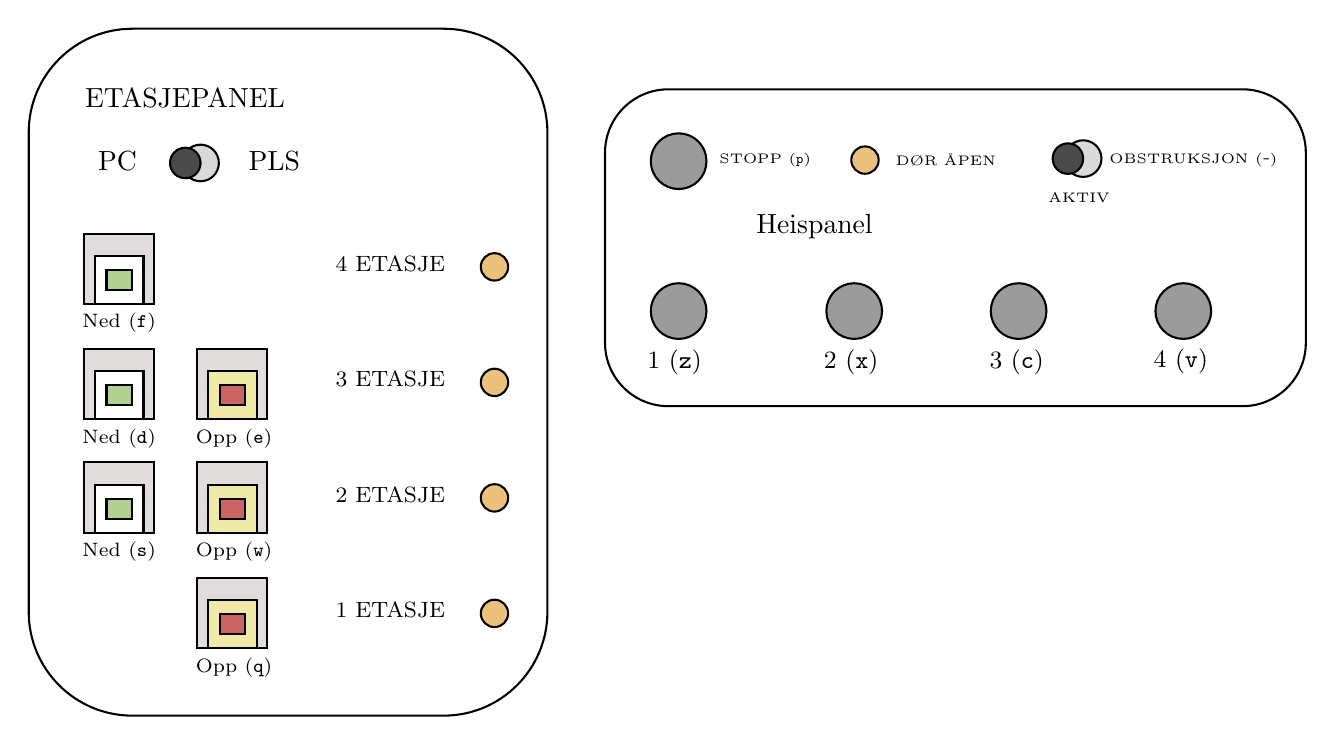
\begin{tikzpicture}[x=0.75pt,y=0.75pt,yscale=-1.05,xscale=1.05]
%uncomment if require: \path (0,386); %set diagram left start at 0, and has height of 386

%Rounded Rect [id:dp9950110832791259] 
\draw   (47.56,88.6) .. controls (47.56,62.31) and (68.87,41) .. (95.16,41) -- (237.96,41) .. controls (264.25,41) and (285.56,62.31) .. (285.56,88.6) -- (285.56,308.6) .. controls (285.56,334.89) and (264.25,356.2) .. (237.96,356.2) -- (95.16,356.2) .. controls (68.87,356.2) and (47.56,334.89) .. (47.56,308.6) -- cycle ;
%Shape: Circle [id:dp32702530949930675] 
\draw  [fill={rgb, 255:red, 219; green, 218; blue, 218 }  ,fill opacity=1 ] (118,102.6) .. controls (118,97.96) and (121.76,94.2) .. (126.4,94.2) .. controls (131.04,94.2) and (134.8,97.96) .. (134.8,102.6) .. controls (134.8,107.24) and (131.04,111) .. (126.4,111) .. controls (121.76,111) and (118,107.24) .. (118,102.6) -- cycle ;
%Shape: Circle [id:dp5550022005610891] 
\draw  [fill={rgb, 255:red, 74; green, 74; blue, 74 }  ,fill opacity=1 ] (112.4,102.6) .. controls (112.4,98.73) and (115.53,95.6) .. (119.4,95.6) .. controls (123.27,95.6) and (126.4,98.73) .. (126.4,102.6) .. controls (126.4,106.47) and (123.27,109.6) .. (119.4,109.6) .. controls (115.53,109.6) and (112.4,106.47) .. (112.4,102.6) -- cycle ;
%Rounded Rect [id:dp07742975412184872] 
\draw   (312,97.88) .. controls (312,81.82) and (325.02,68.8) .. (341.08,68.8) -- (604.48,68.8) .. controls (620.54,68.8) and (633.56,81.82) .. (633.56,97.88) -- (633.56,185.12) .. controls (633.56,201.18) and (620.54,214.2) .. (604.48,214.2) -- (341.08,214.2) .. controls (325.02,214.2) and (312,201.18) .. (312,185.12) -- cycle ;
%Shape: Circle [id:dp5584647222054995] 
\draw  [fill={rgb, 255:red, 155; green, 155; blue, 155 }  ,fill opacity=1 ] (333,101.78) .. controls (333,94.72) and (338.72,89) .. (345.78,89) .. controls (352.84,89) and (358.56,94.72) .. (358.56,101.78) .. controls (358.56,108.84) and (352.84,114.56) .. (345.78,114.56) .. controls (338.72,114.56) and (333,108.84) .. (333,101.78) -- cycle ;
%Shape: Circle [id:dp36378536676727435] 
\draw  [fill={rgb, 255:red, 235; green, 193; blue, 124 }  ,fill opacity=1 ] (425,101.28) .. controls (425,97.81) and (427.81,95) .. (431.28,95) .. controls (434.75,95) and (437.56,97.81) .. (437.56,101.28) .. controls (437.56,104.75) and (434.75,107.56) .. (431.28,107.56) .. controls (427.81,107.56) and (425,104.75) .. (425,101.28) -- cycle ;
%Shape: Circle [id:dp2626490795793748] 
\draw  [fill={rgb, 255:red, 219; green, 218; blue, 218 }  ,fill opacity=1 ] (523,100.6) .. controls (523,95.96) and (526.76,92.2) .. (531.4,92.2) .. controls (536.04,92.2) and (539.8,95.96) .. (539.8,100.6) .. controls (539.8,105.24) and (536.04,109) .. (531.4,109) .. controls (526.76,109) and (523,105.24) .. (523,100.6) -- cycle ;
%Shape: Circle [id:dp7325663462799819] 
\draw  [fill={rgb, 255:red, 74; green, 74; blue, 74 }  ,fill opacity=1 ] (517.4,100.6) .. controls (517.4,96.73) and (520.53,93.6) .. (524.4,93.6) .. controls (528.27,93.6) and (531.4,96.73) .. (531.4,100.6) .. controls (531.4,104.47) and (528.27,107.6) .. (524.4,107.6) .. controls (520.53,107.6) and (517.4,104.47) .. (517.4,100.6) -- cycle ;

%Shape: Circle [id:dp3804510595811603] 
\draw  [fill={rgb, 255:red, 155; green, 155; blue, 155 }  ,fill opacity=1 ] (333,170.56) .. controls (333,163.5) and (338.72,157.78) .. (345.78,157.78) .. controls (352.84,157.78) and (358.56,163.5) .. (358.56,170.56) .. controls (358.56,177.62) and (352.84,183.34) .. (345.78,183.34) .. controls (338.72,183.34) and (333,177.62) .. (333,170.56) -- cycle ;
%Shape: Circle [id:dp9317202699472626] 
\draw  [fill={rgb, 255:red, 155; green, 155; blue, 155 }  ,fill opacity=1 ] (413.56,170.56) .. controls (413.56,163.5) and (419.28,157.78) .. (426.34,157.78) .. controls (433.4,157.78) and (439.12,163.5) .. (439.12,170.56) .. controls (439.12,177.62) and (433.4,183.34) .. (426.34,183.34) .. controls (419.28,183.34) and (413.56,177.62) .. (413.56,170.56) -- cycle ;
%Shape: Circle [id:dp8967657062909633] 
\draw  [fill={rgb, 255:red, 155; green, 155; blue, 155 }  ,fill opacity=1 ] (489,170.56) .. controls (489,163.5) and (494.72,157.78) .. (501.78,157.78) .. controls (508.84,157.78) and (514.56,163.5) .. (514.56,170.56) .. controls (514.56,177.62) and (508.84,183.34) .. (501.78,183.34) .. controls (494.72,183.34) and (489,177.62) .. (489,170.56) -- cycle ;
%Shape: Circle [id:dp46875668862956843] 
\draw  [fill={rgb, 255:red, 155; green, 155; blue, 155 }  ,fill opacity=1 ] (564.56,170.56) .. controls (564.56,163.5) and (570.28,157.78) .. (577.34,157.78) .. controls (584.4,157.78) and (590.12,163.5) .. (590.12,170.56) .. controls (590.12,177.62) and (584.4,183.34) .. (577.34,183.34) .. controls (570.28,183.34) and (564.56,177.62) .. (564.56,170.56) -- cycle ;
%Shape: Circle [id:dp6506882141668844] 
\draw  [fill={rgb, 255:red, 235; green, 193; blue, 124 }  ,fill opacity=1 ] (255,150.28) .. controls (255,146.81) and (257.81,144) .. (261.28,144) .. controls (264.75,144) and (267.56,146.81) .. (267.56,150.28) .. controls (267.56,153.75) and (264.75,156.56) .. (261.28,156.56) .. controls (257.81,156.56) and (255,153.75) .. (255,150.28) -- cycle ;
%Shape: Circle [id:dp7349408120329506] 
\draw  [fill={rgb, 255:red, 235; green, 193; blue, 124 }  ,fill opacity=1 ] (255,203.28) .. controls (255,199.81) and (257.81,197) .. (261.28,197) .. controls (264.75,197) and (267.56,199.81) .. (267.56,203.28) .. controls (267.56,206.75) and (264.75,209.56) .. (261.28,209.56) .. controls (257.81,209.56) and (255,206.75) .. (255,203.28) -- cycle ;
%Shape: Circle [id:dp08591264771647289] 
\draw  [fill={rgb, 255:red, 235; green, 193; blue, 124 }  ,fill opacity=1 ] (255,256.28) .. controls (255,252.81) and (257.81,250) .. (261.28,250) .. controls (264.75,250) and (267.56,252.81) .. (267.56,256.28) .. controls (267.56,259.75) and (264.75,262.56) .. (261.28,262.56) .. controls (257.81,262.56) and (255,259.75) .. (255,256.28) -- cycle ;
%Shape: Circle [id:dp13492097445361106] 
\draw  [fill={rgb, 255:red, 235; green, 193; blue, 124 }  ,fill opacity=1 ] (255,309.28) .. controls (255,305.81) and (257.81,303) .. (261.28,303) .. controls (264.75,303) and (267.56,305.81) .. (267.56,309.28) .. controls (267.56,312.75) and (264.75,315.56) .. (261.28,315.56) .. controls (257.81,315.56) and (255,312.75) .. (255,309.28) -- cycle ;
%Shape: Square [id:dp9156786654213831] 
\draw  [fill={rgb, 255:red, 226; green, 221; blue, 221 }  ,fill opacity=1 ] (72.8,135) -- (105,135) -- (105,167.2) -- (72.8,167.2) -- cycle ;
%Shape: Rectangle [id:dp9366523430197387] 
\draw  [color={rgb, 255:red, 0; green, 0; blue, 0 }  ,draw opacity=1 ][fill={rgb, 255:red, 255; green, 255; blue, 255 }  ,fill opacity=1 ] (77.8,145.2) -- (100.24,145.2) -- (100.24,167.2) -- (77.8,167.2) -- cycle ;
%Shape: Rectangle [id:dp17647947769063999] 
\draw  [fill={rgb, 255:red, 177; green, 207; blue, 144 }  ,fill opacity=1 ] (83.24,151.6) -- (94.8,151.6) -- (94.8,160.8) -- (83.24,160.8) -- cycle ;
%Shape: Square [id:dp3110641273660344] 
\draw  [fill={rgb, 255:red, 226; green, 221; blue, 221 }  ,fill opacity=1 ] (124.8,188) -- (157,188) -- (157,220.2) -- (124.8,220.2) -- cycle ;
%Shape: Rectangle [id:dp3411082188269683] 
\draw  [fill={rgb, 255:red, 240; green, 234; blue, 168 }  ,fill opacity=1 ] (129.8,198.2) -- (152.24,198.2) -- (152.24,220.2) -- (129.8,220.2) -- cycle ;
%Shape: Rectangle [id:dp024921669891114773] 
\draw  [fill={rgb, 255:red, 204; green, 100; blue, 100 }  ,fill opacity=1 ] (135.24,204.6) -- (146.8,204.6) -- (146.8,213.8) -- (135.24,213.8) -- cycle ;
%Shape: Square [id:dp802085856449118] 
\draw  [fill={rgb, 255:red, 226; green, 221; blue, 221 }  ,fill opacity=1 ] (124.8,240) -- (157,240) -- (157,272.2) -- (124.8,272.2) -- cycle ;
%Shape: Rectangle [id:dp5915145699519246] 
\draw  [fill={rgb, 255:red, 240; green, 234; blue, 168 }  ,fill opacity=1 ] (129.8,250.2) -- (152.24,250.2) -- (152.24,272.2) -- (129.8,272.2) -- cycle ;
%Shape: Rectangle [id:dp03960973210916041] 
\draw  [fill={rgb, 255:red, 204; green, 100; blue, 100 }  ,fill opacity=1 ] (135.24,256.6) -- (146.8,256.6) -- (146.8,265.8) -- (135.24,265.8) -- cycle ;
%Shape: Square [id:dp831298532737776] 
\draw  [fill={rgb, 255:red, 226; green, 221; blue, 221 }  ,fill opacity=1 ] (124.8,293) -- (157,293) -- (157,325.2) -- (124.8,325.2) -- cycle ;
%Shape: Rectangle [id:dp15467787894146512] 
\draw  [fill={rgb, 255:red, 240; green, 234; blue, 168 }  ,fill opacity=1 ] (129.8,303.2) -- (152.24,303.2) -- (152.24,325.2) -- (129.8,325.2) -- cycle ;
%Shape: Rectangle [id:dp34679432751904793] 
\draw  [fill={rgb, 255:red, 204; green, 100; blue, 100 }  ,fill opacity=1 ] (135.24,309.6) -- (146.8,309.6) -- (146.8,318.8) -- (135.24,318.8) -- cycle ;
%Shape: Square [id:dp4723272264815428] 
\draw  [fill={rgb, 255:red, 226; green, 221; blue, 221 }  ,fill opacity=1 ] (72.8,240) -- (105,240) -- (105,272.2) -- (72.8,272.2) -- cycle ;
%Shape: Rectangle [id:dp07462637657852489] 
\draw  [color={rgb, 255:red, 0; green, 0; blue, 0 }  ,draw opacity=1 ][fill={rgb, 255:red, 255; green, 255; blue, 255 }  ,fill opacity=1 ] (77.8,250.2) -- (100.24,250.2) -- (100.24,272.2) -- (77.8,272.2) -- cycle ;
%Shape: Rectangle [id:dp5263621720064795] 
\draw  [fill={rgb, 255:red, 177; green, 207; blue, 144 }  ,fill opacity=1 ] (83.24,256.6) -- (94.8,256.6) -- (94.8,265.8) -- (83.24,265.8) -- cycle ;
%Shape: Square [id:dp4171956285217089] 
\draw  [fill={rgb, 255:red, 226; green, 221; blue, 221 }  ,fill opacity=1 ] (72.8,188) -- (105,188) -- (105,220.2) -- (72.8,220.2) -- cycle ;
%Shape: Rectangle [id:dp8897782495872741] 
\draw  [color={rgb, 255:red, 0; green, 0; blue, 0 }  ,draw opacity=1 ][fill={rgb, 255:red, 255; green, 255; blue, 255 }  ,fill opacity=1 ] (77.8,198.2) -- (100.24,198.2) -- (100.24,220.2) -- (77.8,220.2) -- cycle ;
%Shape: Rectangle [id:dp3645531927882917] 
\draw  [fill={rgb, 255:red, 177; green, 207; blue, 144 }  ,fill opacity=1 ] (83.24,204.6) -- (94.8,204.6) -- (94.8,213.8) -- (83.24,213.8) -- cycle ;

% Text Node
\draw (72,67) node [anchor=north west][inner sep=0.75pt]   [align=left] {ETASJEPANEL};
% Text Node
\draw (78,96) node [anchor=north west][inner sep=0.75pt]   [align=left] {PC};
% Text Node
\draw (147,96) node [anchor=north west][inner sep=0.75pt]   [align=left] {PLS};
% Text Node
\draw (380.05,124.81) node [anchor=north west][inner sep=0.75pt]   [align=left] {Heispanel};
% Text Node
\draw (444.05,96.81) node [anchor=north west][inner sep=0.75pt]  [font=\tiny] [align=left] {DØR ÅPEN};
% Text Node
\draw (542.05,96.81) node [anchor=north west][inner sep=0.75pt]  [font=\tiny] [align=left] {OBSTRUKSJON (\verb|-|)};
% Text Node
\draw (363.05,96.81) node [anchor=north west][inner sep=0.75pt]  [font=\tiny] [align=left] {STOPP (\verb|p|)};
% Text Node
\draw (514.05,114.81) node [anchor=north west][inner sep=0.75pt]  [font=\tiny] [align=left] {AKTIV};
% Text Node
\draw (330.05,186.81) node [anchor=north west][inner sep=0.75pt]  [font=\small] [align=left] {1 (\verb|z|)};
% Text Node
\draw (411.05,186.81) node [anchor=north west][inner sep=0.75pt]  [font=\small] [align=left] {2 (\verb|x|)};
% Text Node
\draw (487.05,186.81) node [anchor=north west][inner sep=0.75pt]  [font=\small] [align=left] {3 (\verb|c|)};
% Text Node
\draw (562.34,186.34) node [anchor=north west][inner sep=0.75pt]  [font=\small] [align=left] {4 (\verb|v|)};
% Text Node
\draw (187,144) node [anchor=north west][inner sep=0.75pt]  [font=\footnotesize] [align=left] {4 ETASJE};
% Text Node
\draw (187,197) node [anchor=north west][inner sep=0.75pt]  [font=\footnotesize] [align=left] {3 ETASJE};
% Text Node
\draw (187,250) node [anchor=north west][inner sep=0.75pt]  [font=\footnotesize] [align=left] {2 ETASJE};
% Text Node
\draw (187,303) node [anchor=north west][inner sep=0.75pt]  [font=\footnotesize] [align=left] {1 ETASJE};
% Text Node
\draw (70.8,170.2) node [anchor=north west][inner sep=0.75pt]  [font=\scriptsize] [align=left] {Ned (\verb|f|)};
% Text Node
\draw (70.8,223.2) node [anchor=north west][inner sep=0.75pt]  [font=\scriptsize] [align=left] {Ned (\verb|d|)};
% Text Node
\draw (70.8,275.2) node [anchor=north west][inner sep=0.75pt]  [font=\scriptsize] [align=left] {Ned (\verb|s|)};
% Text Node
\draw (122.8,223.2) node [anchor=north west][inner sep=0.75pt]  [font=\scriptsize] [align=left] {Opp (\verb|e|)};
% Text Node
\draw (122.8,275.2) node [anchor=north west][inner sep=0.75pt]  [font=\scriptsize] [align=left] {Opp (\verb|w|)};
% Text Node
\draw (122.8,328.2) node [anchor=north west][inner sep=0.75pt]  [font=\scriptsize] [align=left] {Opp (\verb|q|)};


\end{tikzpicture}
    \caption{Etasje- og Heispanel i heissimulatoren.}
    \label{fig:paneler_simulator}
\end{figure}

\section{Appendiks - Kodekvalitet}\label{sec:app-kodekval}



Kodekvalitet er et mål på hvor lesbar og \textit{åpenbar} koden er. Koden er lesbar om man er i stand til å ta en snutt og si nøyaktig hva den gjør, og hvorfor den gjør det, basert på koden alene. For deres egen del bør dere derfor alltid ha kodekvalitet i bakhodet hele tiden. Felles for god kode er at det resulterer i en lesbar kode som er lettere å vedlikeholde enn mindre god kode. 

Ute i virkelige settinger bruker man mye mer tid på å lese kode enn å skrive kode selv. Uavhengig om det er noen andre sin kode kode, eller deres egen kode en del frem i tid, er det mye greiere om den er skrevet for leserens skyld - enn at den er skrevet for å spare nanosekunder på ubetydelige steder.

Under er det oppgitt en liste av hva som regnes som god kodekvalitet i dette faget. Listen er i  stor grad basert på \textit{Code Complete 2} av Steve McConnell, men noen ekstra punkter som er nyttige for \verb|C| er også lagt til. Det er helt greit å være uenig i deler av- eller hele listen, men da bør man ha en god konvensjon som man bruker konsekvent.




\subsection{Moduler}

\begin{itemize}
    \item Alle funksjonene i en modul bør ha samme abstraksjonsnivå. Man burde aldri blande lav-nivå funksjonalitet med høy-nivå funksjonalitet.
    \item En modul har som formål å gjemme noe bak et grensesnitt. Det bør altså ikke lekke ut detaljer om modulens implementasjon til overflaten. Ideelt sett skal man kunne bruke modulen uten å vite om hvordan modulen var implementert.
    
    \item Hver modul skal ha en sentral oppgave. En modul bør dermed ikke håndtere flere vidt forskjellige ansvarsområder.
    
    \item Grensesnittet til hver modul bør gjøre det helt åpenbart hvordan modulen skal brukes. I dette ligger det også å navngi modul-funksjoner logisk og presist.
    
    \item Moduler bør snakke med så få andre moduler som mulig, og samarbeidet mellom moduler bær være så lett koblet som mulig. Dere skal altså kunne fjerne en modul, uten å måtte endre på alle andre som inngår i programmet. 
    
    \item For klasser er det ønskelig at alle medlems-variabler er definerte etter at konstruktøren har kjørt. Tilsvarende for moduler er det ønskelig at all medlemsdata er definert etter en eventuell initialiseringsfunksjon.
\end{itemize}



\subsection{Funksjoner}

\begin{itemize}
    \item Den viktigste grunnen til å opprette en funksjon er ikke kodegjenbruk, men å gi brukeren en måte å håndtere kompleksitet på. Det er tilfeller hvor det faktisk er mer lesbart å repetere dere selv et par ganger, fremfor å trekke noen få linjer ut i en egen funksjon.
    
    \item Alle funksjoner bør ha ett eneste ansvarsområde - en oppgave som funksjonen gjør bra.
    
    \item Navnet på en funksjon bør beskrive alt funksjonen gjør.
    
    \item Sterke verb foretrekkes fremfor svake- og vage verb. For eksempel bør dere sky ord som \verb|handle| eller \verb|manage|.
    
    \item Kohesjon er et viktig begrep for å klassifisere funksjoner:
    \begin{outline}
    \1 \textbf{Sekvensiell kohesjon} beskriver funksjoner hvor stegene som tas innad i funksjonen må gjøres i den bestemte rekkefølgen de er satt opp i.
    \1 \textbf{Kommunikasjons-kohesjon} er når en funksjon benytter samme data til å gjøre forskjellige ting, men hvor bruken av data-en ellers er urelatert.
    \1 \textbf{Tidsavhengig kohesjon} har man hvis en funksjon inneholder mange forskjellige operasjoner som gjøres til samme tid, men som ellers ikke har noe med hverandre å gjøre.
    
    \1 \textbf{Funksjonell kohesjon} har man i funksjoner hvor instruksjonene som kalles samarbeider for å gjøre en og samme ting. Tingene funksjonen gjør er altså nødvendige for å utføre en bestemt oppgave.
\end{outline}

    Av disse er det mest ønskelig å ha funksjonell kohesjon.
    

    \item Motsatte verb, bør være presise og opptre i veldefinerte par som: \verb|begin| - \verb|end|, \verb|create| - \verb|destroy|, \verb|open| - \verb|close| eller \verb|next| - \verb|previous|
    
    \item Funksjoner bør være \textit{self-contained}, slik at de til en liten grad avhenger av returverdien til andre funksjoner. Om dette ikke er mulig, bør denne koblingen være så løs som mulig slik at man ikke trenger å endre mange andre funksjoner når man skal modifisere en spesifikk funksjon.
\end{itemize}



\subsection{Variabler}

\begin{itemize}
    \item Unngå å bruke for mange \textit{arbeids-variabler} - variabler som opprettes i starten av en funksjon for så å muteres gjennom hele funksjonens levetid.
    \item Navnekvaliteten til en variabel bør speile variabelens levetid. Variabler som brukes til å itere en løkke kan hete \verb|i|, mens en global variabel bør ha et virkelig godt navn som presist beskriver variabelen.
\end{itemize}

\subsection{Kommentarer}

\begin{itemize}
    \item Når man kommenterer kode, er det en erkjennelse om at koden som kommentaren beskriver ikke er åpenbar. Åpenbar kode som forklarer seg selv trenger ikke kommentarer, og er bedre enn uklar kode med kommentarer.
    \item Alle kommentarer må være oppdatert. Det er fort gjort å endre kode, uten å endre kommentarene rundt. Kode med ukorrekte kommentarer har mindre verdi enn kode uten kommentarer.
\end{itemize}

\subsection{Øvrig}

\begin{itemize}
    \item Funksjoner bør prefikses med navnet på modulen sin for å gjøre det åpenbart hvor funksjonen kommer fra, og for å gjøre samme jobb som et namespace.
    \item Variabler kan med fordel prefikses med \verb|p_| om de er pekere, \verb|pp_| om de er pekere til pekere, \verb|m_| om de er modul-variabler begrenset med kodeordet \verb|static|, og \verb|g_| om de er globale.
    
    \item Forkortelser er greit å bruke såfremt de er veletablerte. Et eksempel på veletablert forkortelse er \verb|FSM| (finite-state machine = tilstandsmaskin). For eksempel: forkortelser av typen \verb|EHM| for "etasjehåndteringsmodul" bør unngås.
    
    
    
    \item Selv om \verb|C| er forholdsvis lavnivå er det fullt mulig å ivareta god softewareutviklingspraksis. Allikevel kommer man alltid til å skrive noe \textit{uggen} kode - det gjelder bare å velge det beste alternativet tilgjengelig.
    
    \item Det er helt greit å være uenig i denne listen, eller ha andre konvensjoner dere vil heller følge, så lenge dette kan argumenteres for at de gir god lesbarhet og vedlikeholdbarhet.
\end{itemize}

% \section{Appendiks - Git-historikk}\label{sec:app-git}
% Bruk git slik beskrevet i øving 2. Bruk valgfri 